\documentclass[a4paper,twoside]{article}

\usepackage{epsfig}
\usepackage{subfigure}
\usepackage{calc}
\usepackage{amssymb}
\usepackage{amstext}
\usepackage{amsmath}
\usepackage{amsthm}
\usepackage{multicol}
\usepackage{pslatex}
\usepackage{subfigure}

\usepackage{apalike}
\usepackage{SCITEPRESS}     % Please add other packages that you may need BEFORE the SCITEPRESS.sty package.

\subfigtopskip=0pt
\subfigcapskip=0pt
\subfigbottomskip=0pt

\begin{document}

\title{EvoloPy: An open source Nature-Inspired Optimization Toolbox in Python}

\author{\authorname{First Author Name\sup{1}, Second Author Name\sup{1} and Third Author Name\sup{2}}
\affiliation{\sup{1}Institute of Problem Solving, XYZ University, My Street, MyTown, MyCountry}
\affiliation{\sup{2}Department of Computing, Main University, MySecondTown, MyCountry}
\email{\{f\_author, s\_author\}@ips.xyz.edu, t\_author@dc.mu.edu}
}

\keywords{The paper must have at least one keyword. The text must be set to 9-point font size and without the use of bold or italic font style. For more than one keyword, please use a comma as a separator. Keywords must be titlecased.}

\abstract{EvoloPy is an open source and cross-platform Python toolbox that implements a wide range of classical and recent nature-inspired metaheuristic algorithms. The goal of this toolbox is to facilitate the use of metaheuristic algorithms by non-specialists coming from different domains. With a simple interface and minimal dependencies, it is easier for researchers and practitioners to utilize EvoloPy for optimizing and benchmarking their own defined problems using the most powerful metaheuristic optimizers in the literature. On the other hand, the design of this toolbox makes it very easy for the researchers in the domain to integrate their own optimizers and compare their performance to the state of art algorithms. }


\onecolumn \maketitle \normalsize \vfil
\section{\uppercase{Introduction}}

\label{sec:introduction}


Nature-inspired metaheuristic algorithms are considered to be the one of the most efficient approaches to solve optimization problems \cite{Yang_2013}. Nature-inspired metaheuristics imitate natural phenomena such as the the behavior of the nature systems like swarm based algorithms, and evolution based algorithms. Over last three decades, many nature-inspired metaheuristics algorithms have been developed. Swarm intelligence algorithms simulate the natural swarms such as flocks of birds, ant colonies, and schools of fishes such as Particle Swarm Optimization (PSO) \cite{Kennedy95}, Cuckoo Search (CS) \cite{Yang2009}, Ant Colony Optimization (ACO) \cite{Koro_ec_2009}, Grey Wolf Optimizer (GWO) \cite{Mirjalili201446}, Multi-Verse Optimizer (MVO) \cite{Mirjalili2016}, Moth-flame optimization (MFO) \cite{Mirjalili2015228}, Whale Optimization Algorithm (WOA) \cite{Mirjalili201651}, Bat Algorithm (BA) \cite{Yang2010}, and many others. Most of the previous algorithms reaches the best solutions by exchanging the information between the swarm's individuals. 

On the other hand, evolutionary based algorithms are inspired by some concepts from the Darwinian theories about evolution and natural selection. Such algorithms include Genetic algorithm (GA) \cite{Sivanandam}, Genetic Programming (GP)\cite{Koza1992}, and Evolution Strategy (ES)\cite{Beyer2002}. These algorithms use different strategies to evolve and find good solutions for difficult problems. 

In the last two decades there have been a growing interest in the applications of these algorithms for solving and optimizing complex problems  in different domains.



\section{\uppercase{Related Work}}
Today, there exist many different nature-inspired optimization libraries and toolboxes. Some of them are developed for special type of nature-inspired optimization like GEATbx \cite{GEATbx}, which is a toolbox contains many variants of the genetic algorithms, and genetic Programming. GEATbx is implemented in MATLAB environment and provides many global optimization capabilities. The authors in \cite {GAlib} developed GAlib library, which contains a set of C++ genetic algorithm tools and operators for different optimization problems. GAlib is built on UNIX platforms and supported parallel experiments. In \cite {DEAP_JMLR2012}, the authors developed a novel evolutionary computation python framework called DEAP to simplify the execution of many optimization ideas with  parallelisation features. The DEAP Framework includes many nature-inspired algorithms with different variations such as: Genetic Algorithm, Genetic Programing (GP), Evolution Strategies (ES), Particle Swarm Optimization (PSO), Differential Evolution (DE), and multi-objective optimization. In addition, Deap includes Benchmarks modules containing many test functions for evaluations. In \cite{Wagner04}, the author presents a generic optimization environment named HeuristicLab. HeuristicLab is a framework for heuristic, evolutionary algorithms, and machine learning. HeuristicLab includes many algorithms such as: Genetic Programming, Age-layered Population, Structure (ALPS), Evolution Strategy, Genetic Algorithm, Island Genetic Algorithm, Particle Swarm Optimization, Relevant Alleles Preserving GA, and many others.





\section{\uppercase{Why Python?}}

Python is a general purpose scripting language which has a clear and simple syntax. With the rapid development of mature, advanced  and open source scientific computing libraries and packages, Python became as one of the most popular and powerful languages for scientific computing.
Moreover, Python has cross-platform runability, which works with different operating systems, and has ability to access libraries written in different programming languages and computing environments. Python also can support small-form devices, embedded systems, and microcontrollers. In addition, Python needs very minimal setup procedure to start with. Python uses modular and object based programming, which is a popular methodology to organize classes, functions, and procedures into hierarchical namespaces. All these reason has turned Python to be a popular language in a huge community of scientists. 



\section{Design issues}

Most of nature inspired metaheuristics are population-based algorithms. These algorithms start by randomly initializing a set of individuals each of which represents a candidate solution. Conventionally, in most of state-of-art evolutionary algorithms frameworks, populations are implemented as 2-dimensional arrays while individuals are implemented as 1-dimensional array. For example an individual $I$ and a population $P$ can be represented as given in equations \ref{eq:individual} and \ref{eq:population}.

\begin{equation}
I_{i}=[\begin{array}{cccc}
x_{i}^{1} & x_{i}^{2} & ... & x_{i}^{d}\end{array}]
\label{eq:individual}
\end{equation}

\begin{equation}
P=\left[\begin{array}{cccc}
x_{1}^{1} & x_{1}^{2} & ... & x_{1}^{d}\\
x_{2}^{1} & x_{2}^{2} & ... & x_{2}^{d}\\
\vdots & \vdots & \vdots & \vdots\\
x_{n}^{1} & x_{n}^{2} & ... & x_{n}^{d}
\end{array}\right]
\label{eq:population}
\end{equation}

In EvoloPy, \texttt{Numpy} is chosen to define and represent the populations and individuals in the optimizers. Numpy library is one of the main packages for scientific computing in Python. \texttt{Numpy} has many things in common with Matlab. This makes it easier for researchers who are familiar with Matlab use EvoloPy. 

The \texttt{Numpy}’s array class  \texttt{ndarray} is used to define 1-dimensional and 2-dimensional arrays that represent individuals and populations, respectively. For example, to define a randomly generated initial population with 50 individuals and 100 dimensions the following python line of code can be used

\texttt{initialPop = np.random.rand(500,100)}


Moreover, with \texttt{Numpy} it is possible to perform vector operations in simple and compact syntax. For example, a common operation is used in many metaheuristic algorithms is to check the boundaries of the elements of the individuals after updating them. This can be performed all at once with \texttt{Numpy} as follows:

\texttt{newPop=numpy.clip(oldPop, lb, ub)}

Where \texttt{lb} and \texttt{ub} are the upper and lower bounds respectively.

\section{Comparison with Matlab}

In this section we compare the metaheuristic algorithms implemented so far in EvoloPy with their peers in Matlab based on their running time. The idea here is to measure the running time of the main loop of each algorithm in EvoloPy and Matlab with an equal number of function evaluations. The experiments were performed on on a personal machine with an  Intel(R) Core(TM) i5-2400 CPU at 3.10Ghz and a memory of 4 GB running Windows 7 professional 32bit operating system. In all experiments, the population size and the number of iterations was set for all algorithms to 50, and 100, respectively. In order to study the effect of the size of the problem to be solved on the running time of the algorithms, all optimizer are executed using different dimension sizes ranging from a small size of 50 elements reaching up to 20,000 in both implementations, Matlab and EvoloPy. 

\begin{figure*}[H]
\centering

\begin{tabular}{ c c  }
\centering
\subfigure[BAT]{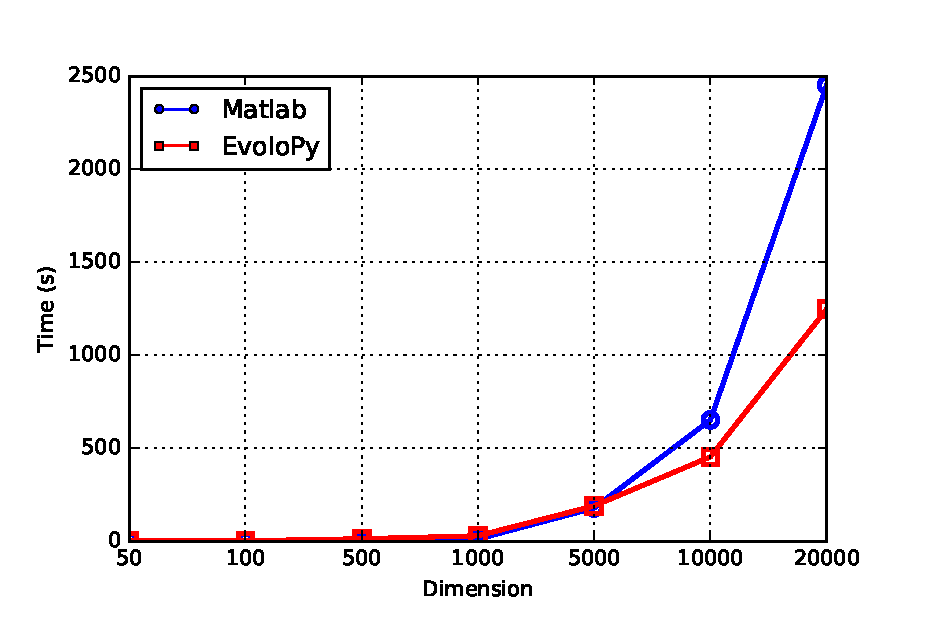
\includegraphics[scale=.45]{BAT.eps}\label{t1}} & 
\subfigure[CS]{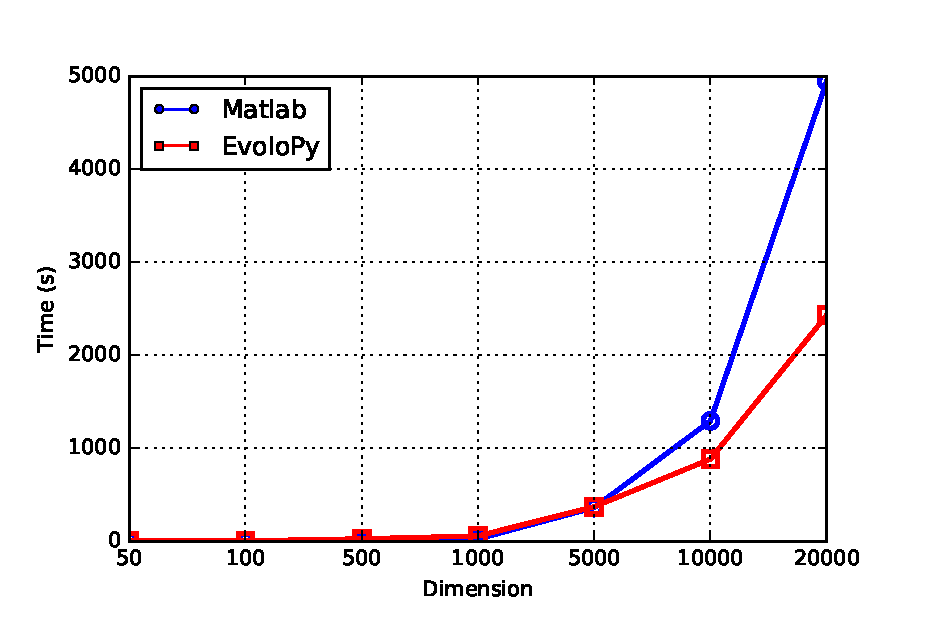
\includegraphics[scale=.45]{CS.eps}} 


\\
\subfigure[FPA]{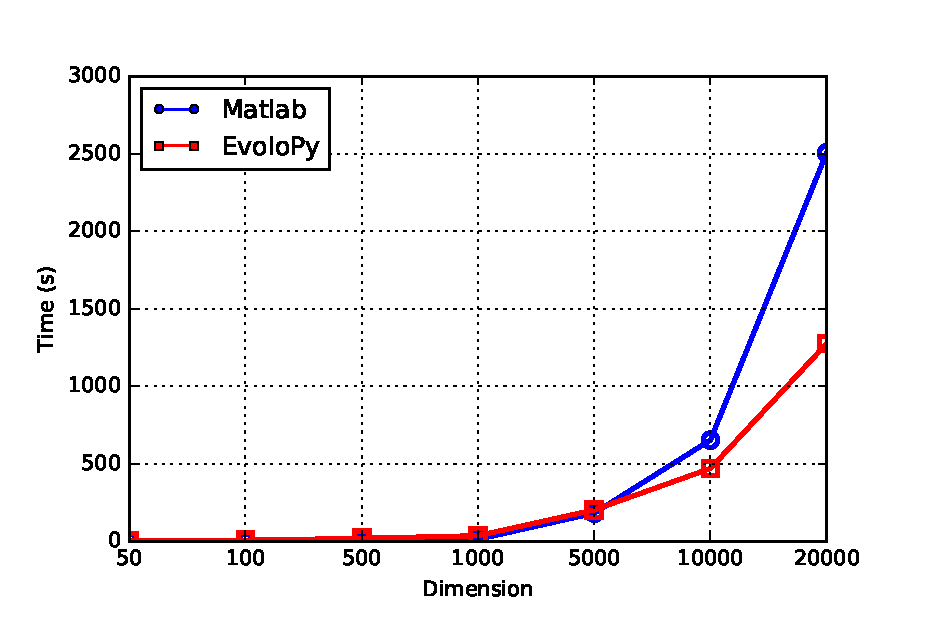
\includegraphics[scale=.45]{FPA}\label{subfigf6t}} & 
\subfigure[GWO]{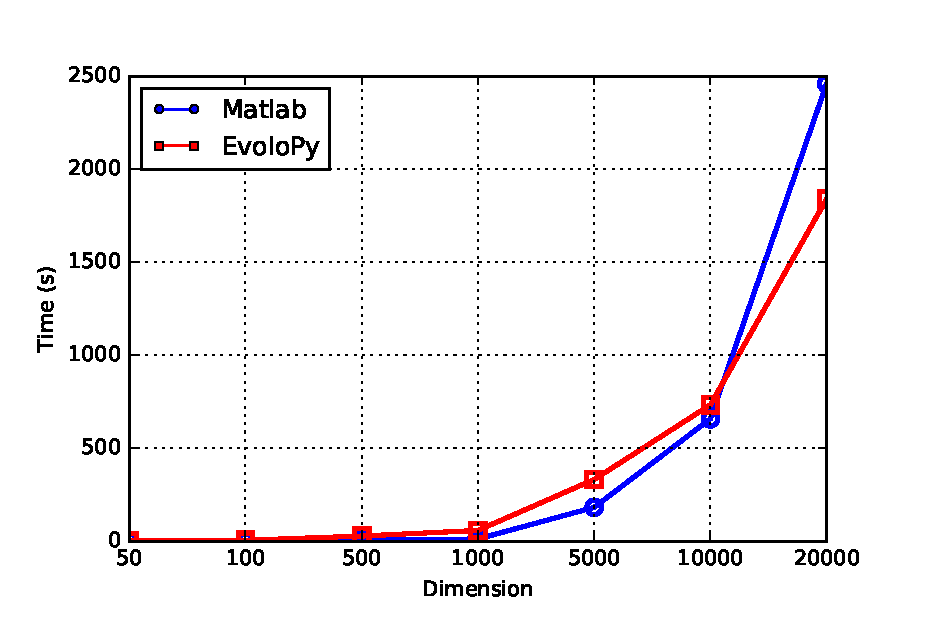
\includegraphics[scale=.45]{GWO}\label{subfigf2s}} 


\\
\subfigure[MFO]{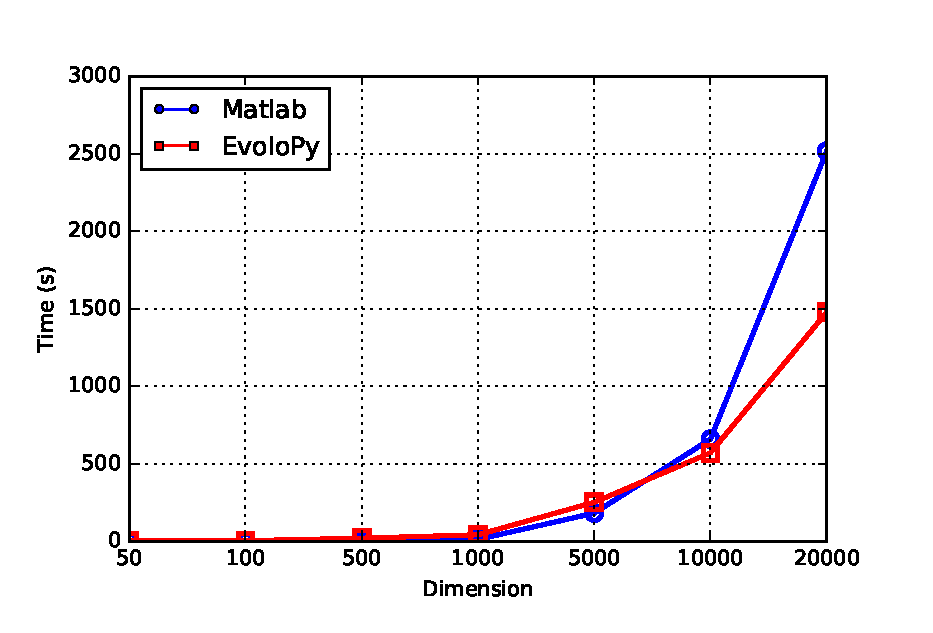
\includegraphics[scale=.45]{MFO.eps}\label{subfigf4s}} & 
\subfigure[MVO]{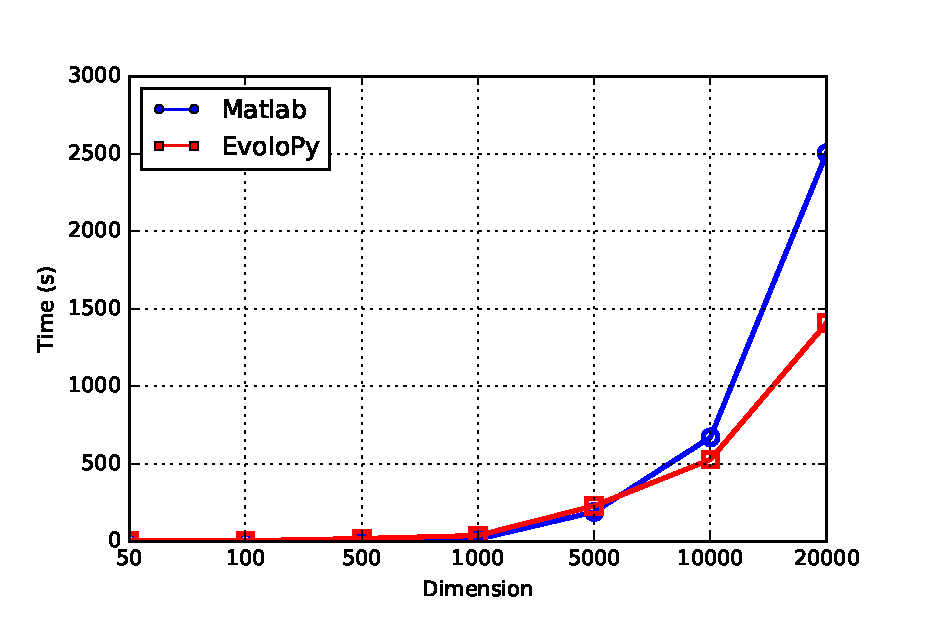
\includegraphics[scale=.45]{MVO.eps}\label{subfigf6s}}

\\

\subfigure[PSO]{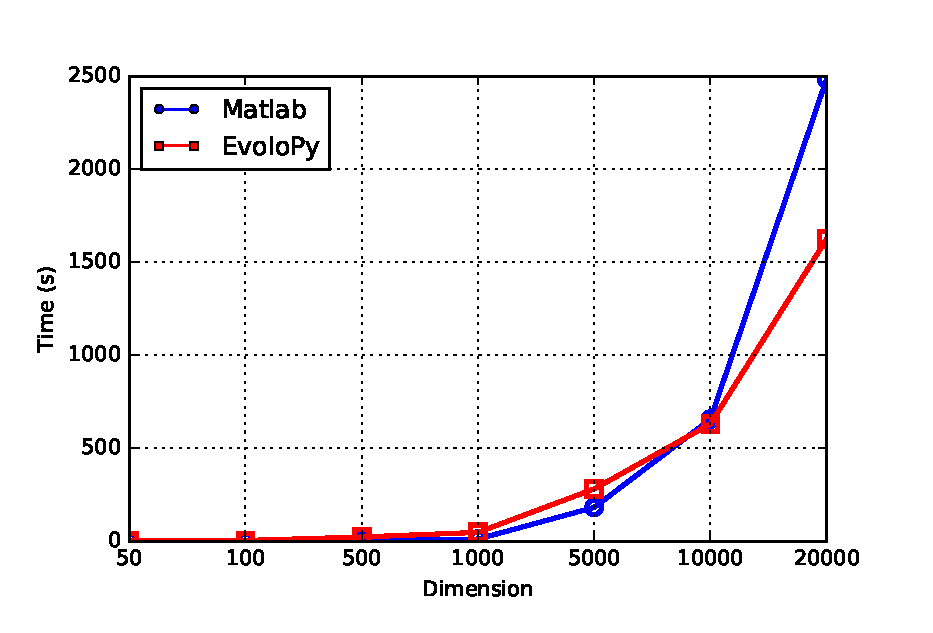
\includegraphics[scale=0.45]{PSO.eps}\label{t2}} &  
\subfigure[WOA]{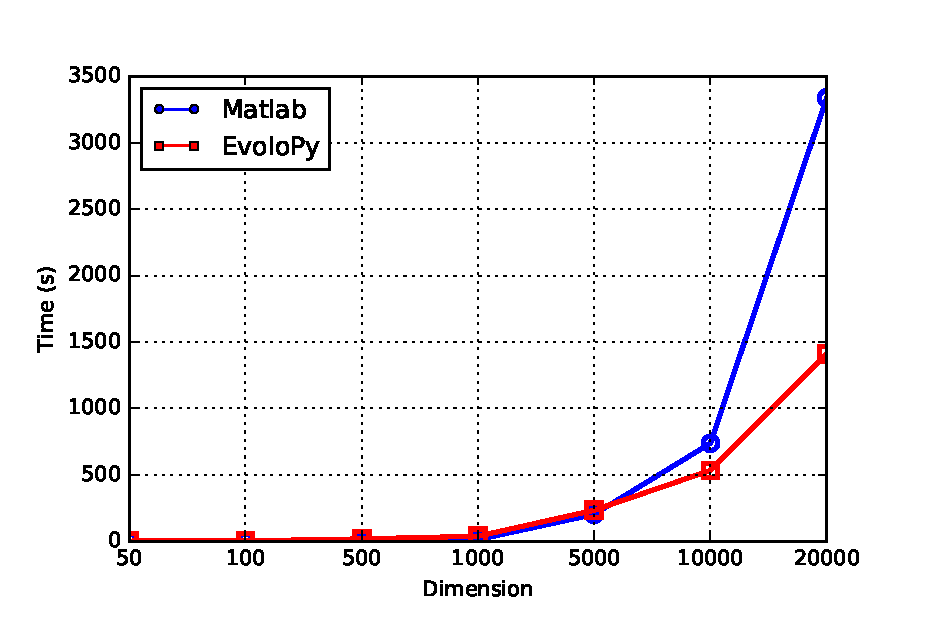
\includegraphics[scale=0.45]{WOA.eps}\label{subfigf4t}} 


\\

\end{tabular}

\caption{Comparison between between the metaheuristic optimizers in EvoloPy and Matlab based on execution time of the main iteration.}
\label{fig:complexity}
\vspace{-0.0in}
\end{figure*}






%\subfigure[Liver]{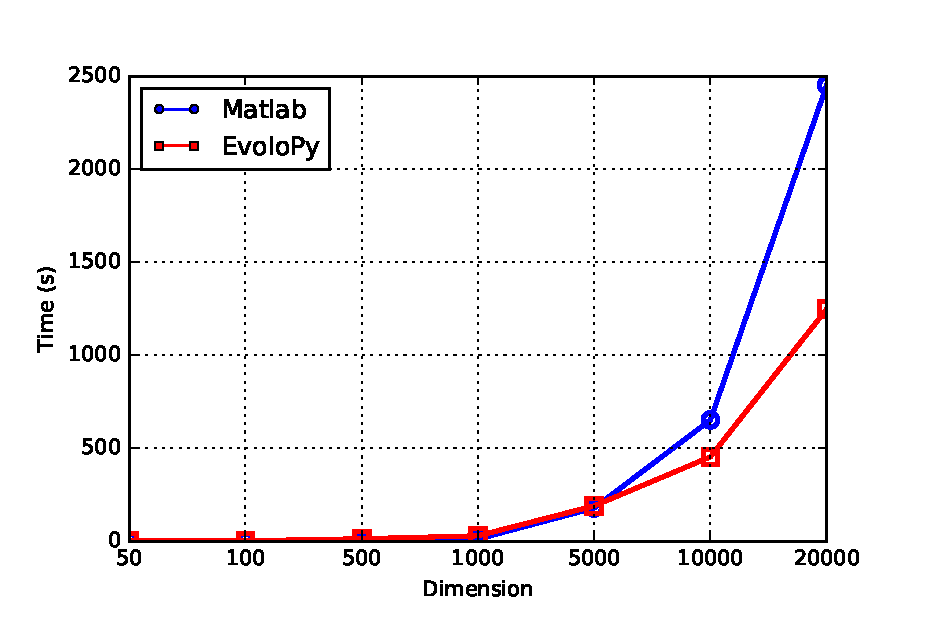
\includegraphics[scale=0.35]{BAT.eps}\label{subfigf6t}} 

\section*{\uppercase{Acknowledgements}}




\vfill
\bibliographystyle{apalike}
{\small
\bibliography{ref}}


\section*{\uppercase{Appendix}}

\noindent If any, 
\textit{$\backslash$section*\{APPENDIX\}}

\vfill
\end{document}

